%% Move the data in this document into another document, ignore the figures before the columns, remove the junk at the bottom of concurrency.
\chapter{CENG 355 CheatSheet}
\definecolor{blizzardblue}{rgb}{0.67, 0.9, 0.93}
\definecolor{burlywood}{rgb}{0.87, 0.72, 0.53}
\definecolor{byzantine}{rgb}{0.74, 0.2, 0.64}
\definecolor{capri}{rgb}{0.0, 0.75, 1.0}
\definecolor{carrotorange}{rgb}{0.93, 0.57, 0.13}
\renewcommand\labelitemi{---}
\setlength{\fboxrule}{2pt}%


% Change to 3 columns for actually cheatsheet
	\begin{figure}
		\centering
		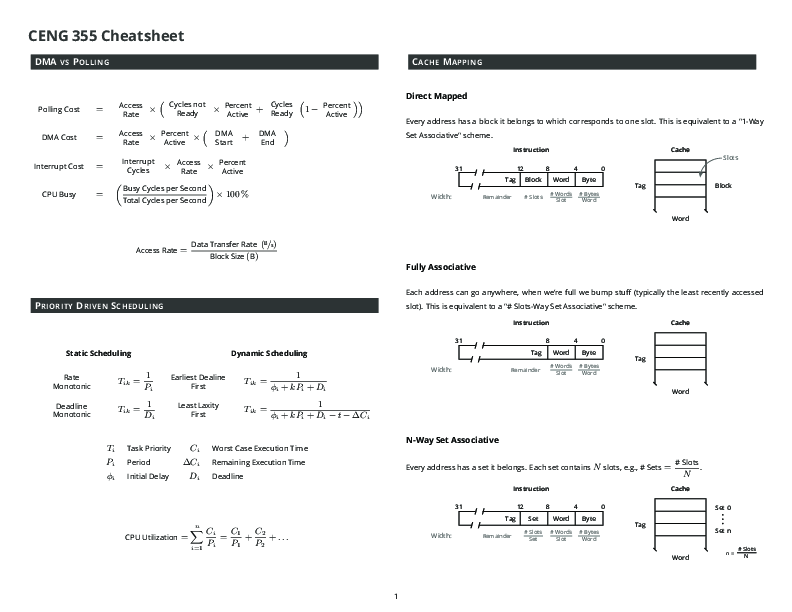
\includegraphics[width=1\linewidth]{CENG355/Ceng355-0.png}
		\caption{Cheatsheet Part 1}
		\label{fig:ceng355-0}
	\end{figure}
	\begin{figure}
		\centering
		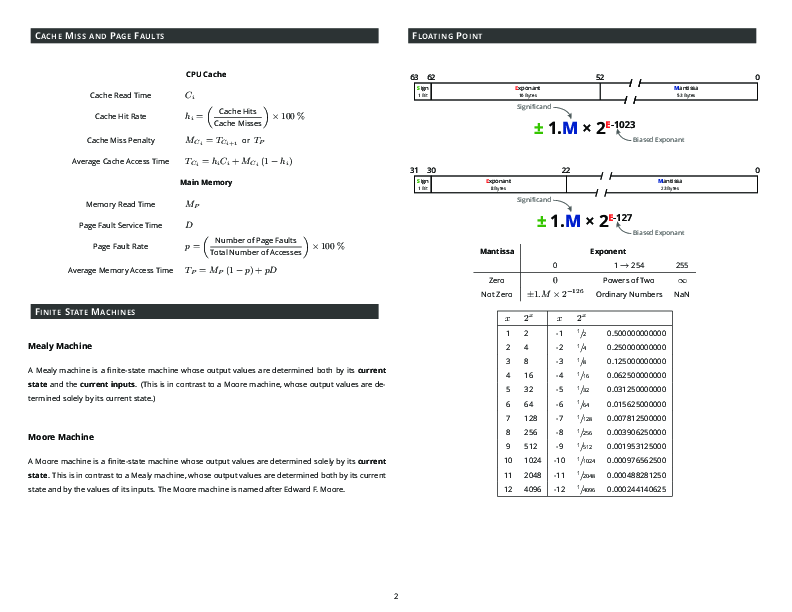
\includegraphics[width=1\linewidth]{CENG355/Ceng355-1.png}
		\caption{CheatSheet Part 2}
		\label{fig:ceng355-1}
	\end{figure}
\begin{multicols}{2}
\section{I/O}
% Create documents for one example from https://www3.nd.edu/~cpoellab/teaching/cse40463/slides4.pdf
\section{Interfacing}
\section{Memory}
\textbf{\underline{Principle of Locality}}:
\hrule
Programs tend to reuse data and instructions near
those they have used recently, or that were recently
referenced themselves. \newline
\textbf{Temporal locality}:
\fcolorbox{byzantine!45}{capri!25}{Recently referenced items are likely to be referenced again in the near future}
\textbf{Spatial locality}:
\fcolorbox{blizzardblue!85}{burlywood!25}{Items with nearby addresses tend to be referenced close together in time.}
\textbf{Data:}
\begin{itemize}
\item Reference array elements in succession: spatial locality
\item Reference sum each iteration: temporal locality
\end{itemize}
\textbf{Instructions:}
\begin{itemize}
\item Reference instructions in sequence: spatial locality.
\item Cycle through loop repeatedly: temporal locality.
\end{itemize}

\subsubsection{Blocked Matrix Code}
\begin{lstlisting}[language=Java]
void bijk(array A, array B, array C, int n, int bsize)
{
	int i, j, k, kk, jj;
	double sum;
	int en = bsize * (n/bsize); /* Amount that fits evenly into blocks */
	
	for (i = 0; i < n; i++)
	for (j = 0; j < n; j++)
	C[i][j] = 0.0;
	
	for (kk = 0; kk < en; kk += bsize) {
		for (jj = 0; jj < en; jj += bsize) {
			for (i = 0; i < n; i++) {
				for (j = jj; j < jj + bsize; j++) {
					sum = C[i][j];
					for (k = kk; k < kk + bsize; k++) {
						sum += A[i][k]*B[k][j];
					}
					C[i][j] = sum;
				}
			}
		}
	}
}
\end{lstlisting}
Copy-paste code here to remove the line numbers.
\end{multicols}
\section{Arithmetic}
\begin{figure}
	\centering
	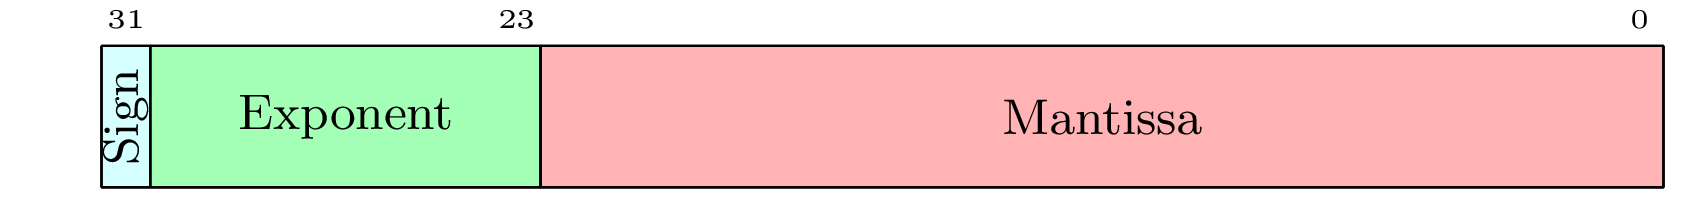
\includegraphics[width=1\linewidth]{CENG355/Exponent.png}
	\caption{IEEE 754 floating point (correct later)}
	\label{fig:exponent}
\end{figure}
\begin{align}
& t_{avg} = h_1C_1 + (1-h_1)(h_2C_2 + (1-h_2)M) \\
& \quad \text{where}  \notag
\end{align}
$h_1$ \textit{is the hit rate in the } $L_1$ \textit{caches.} \newline 
$h_2$ \textit{is the hit rate in the } $L_2$ \textit{ cache.} \newline
$C_1$ \textit{is the time to access information in the } $L_1$ \textit{caches.}\newline
$C_2$ \textit{is the miss penalty to transfer information from the } $L_2$ \text{cache to an } $L_1$ \textit{ cache.} \newline
\textit{M is the miss penalty to transfer information from the main memory to the } $L_2$ \textit{cache.}

\section{Concurrency}

\colorbox{capri!85}{\makebox(12,12){\textcolor{white}{This better work rofl, why is this so damn hard}}}
\setlength{\fboxrule}{6pt}%
\fcolorbox{blizzardblue!85}{carrotorange!85}{Fun with colour} 

\begin{align*}
& \text{Amdahl's Law} =  \frac{1}{f_{unenh} + f_{enh}/p}
\end{align*}

\begin{figure}
	\centering
	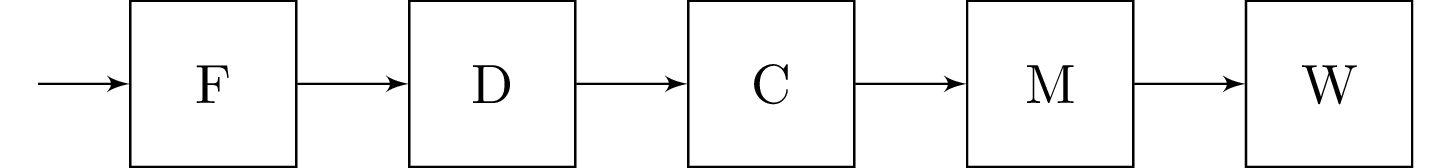
\includegraphics[width=1\linewidth]{CENG355/Pipeline.png}
	\caption{Pipeline for Question 2}
	\label{fig:q2diagram}
\end{figure}
